\documentclass[12pt]{extarticle}
\usepackage{tempora}
\usepackage[T1, T2A]{fontenc}
\usepackage[utf8]{inputenc}
\usepackage[english, ukrainian]{babel}
\usepackage{geometry}
\usepackage{graphicx}
\usepackage{multirow}
\usepackage{multicol}
\usepackage{float}
\usepackage{pgfplots}
\pgfplotsset{width=\textwidth*0.9,compat=1.9}

\graphicspath{{/home/artem/Pictures}}
\geometry
{
    a4paper,
    left=30mm,
    top=15mm,
    right=20mm,
    bottom=15mm,
}

\begin{document}
\begin{titlepage}
    \begin{center}
        \textbf{\normalsize{\MakeUppercase{
            Міністерство Освіти і науки України
            Національний університет "Львівська політехніка"
        }}}

        \begin{flushright}
        \textbf{ІКНІ}\\
        Кафедра \textbf{ПЗ}
        \end{flushright}
        \vspace{15mm}

        \includegraphics[width=0.4\textwidth]{lpnu_logo.png}

        \vspace*{\fill}

        \textbf{\normalsize{\MakeUppercase{Звіт}}}
            
        До лабораторної роботи №7

        \textbf{на тему:} “ЛІНІЙНІ СТРУКТУРИ ДАНИХ”

        \textbf{з дисципліни:} "Алгоритми і структури даних”
            
        \vspace*{\fill}

        \begin{flushright}

            \textbf{Лектор:}\\
            доцент кафедри ПЗ\\
            Коротєєва Т. О.\\
            \vspace{12pt}

            \textbf{Виконав:}\\
            студент групи ПЗ-24\\
            Губик А. С.\\
            \vspace{12pt}

            \textbf{Прийняв:}\\
            асистент кафедри ПЗ\\
            Вишневський О. К.\\
        \vspace{12pt}
        \end{flushright}

        Львів -- 2023
            
            
    \end{center}
\end{titlepage}

\subsection*{Тема роботи} 
ЛІНІЙНІ СТРУКТУРИ ДАНИХ



\subsection*{Мета роботи} Познайомитися з лінійними структурами даних (стек, черга, дек, список) та отримати навички програмування алгоритмів, що їх обробляють.

\subsection*{Індивідуальне завдання}
Варіант 3: односторонній зв’язаний список символів.\\ 

Розробити програму, яка читає з клавіатури послідовність даних, жодне з яких не повторюється, зберігає їх до структури даних (згідно з варіантом), виводить на екран побудовану структуру та наступні характеристики:
\begin{enumerate}
\item       кількість елементів;

\item       мінімальний та максимальний елемент (для символів за кодом);

\item       третій елемент з початку послідовності та другий з кінця послідовності;

\item       елемент, що стоїть перед мінімальним елементом та елемент, що стоїть після максимального;

\item       знайти позицію елемента, значення якого задається з клавіатури;

\item       об'єднати дві структури в одну.
\end{enumerate}

\subsection*{Теоретичні відомості}
Стек, черга, дек, список відносяться до класу лінійних динамічних структур.

 Зі стеку (stack) можна видалити тільки той елемент, який був у нього доданий останнім: стек працює за принципом «останнім прийшов – першим пішов» (last-in, first-out – LIFO).

З черги (queue), навпаки, можна видалити тільки той елемент, який знаходився в черзі довше за всіх: працює принцип «першим прийшов – першим пішов» (first-in, first-out – FIFO).

Дек - це впорядкована лінійна динамічно змінювана послідовність елементів, у якій виконуються такі умови: 1) новий елемент може приєднуватися з обох боків послідовності; 2) вибірка елементів можлива також з обох боків послідовності. Дек називають реверсивною чергою або чергою з двома боками.

У зв’язаному списку (або просто списку; linked list) елементи лінійно впорядковані, але порядок визначається не номерами, як у масиві, а вказівниками, що входять до складу елементів списку. Списки є зручним способом реалізації динамічних множин.

Елемент двобічно зв’язаного списку (doubly linked list) – це запис, що містить три поля: key (ключ) і два вказівники next (наступний) і prev (попередній). Крім цього, елементи списку можуть містити додаткові дані.

У кільцевому списку (circular list) поле prev голови списку вказує на хвіст списку, а поле next хвоста списку вказує на голову списку.

 
\subsection*{{Хід роботи}}
\begin{verbatim}
    #include <iostream>

    struct Node {
        char data;
        Node* next;
    };
    
    class ForwardList {
    private:
        Node* head;
        char max = 0, min = 127;
        size_t size = 0;
    
    public:
        ForwardList() : head(nullptr) {}
    
        void push_front(char value) {
            Node* newNode = new Node;
            newNode->data = value;
            newNode->next = head;
            head = newNode;
            if(value > max) max = value;
            if(value < min) min = value;
            size++;
        }
        int find_pos(char elem){
            Node *tmp = head;
            int i = 0;
            for(; tmp->data != elem; tmp = tmp->next, i++)
            {
                if (tmp->next == nullptr ){
                    i = -1;
                    break;
                }
            }
            return i;
    
        }
        void append(const ForwardList& other) {
            if (other.head == nullptr) {
                return; // Nothing to append
            }
    
            if (head == nullptr) {
                head = new Node{other.head->data, nullptr};
            } else {
                Node* current = head;
                while (current->next != nullptr) {
                    current = current->next;
                }
                current->next = new Node{other.head->data, nullptr};
            }
    
            Node* current = head;
            Node* otherCurrent = other.head->next;
            while (otherCurrent != nullptr) {
                current->next = new Node{otherCurrent->data, nullptr};
                current = current->next;
                otherCurrent = otherCurrent->next;
            }
        }
    
        void print() {
            Node* current = head;
            while (current != nullptr) {
                std::cout << current->data << " ";
                current = current->next;
            }
            std::cout << std::endl;
        }
        void weirdFunction() {
            Node* current = head;
            Node* tmp = head;
            for (int i = 0; i < 2; i++) {
                current = current->next;
            }
            for (int i = 0; i < size - 1; i++) {
                tmp = tmp->next;
            }
            std::cout << "Third element: " << current->data<< std::endl;
            std::cout << "Second from end element: " << tmp->data<< std::endl;
            std::cout << std::endl;
        }
        void strangeFunction() {
            Node* current = head;
            Node* tmp = head;
            int id1 = find_pos(min) - 1;
            int id2 = find_pos(max) + 1;
    
            if(id1 < 0){
                std::cout << "There's no element before min." << std::endl;
            }else{
                for (int i = 0; i < id1; i++)
                {
                    current = current->next;
                }
                std::cout << "Element before min: " << current->data << std::endl;
            }
    
            if(id2 > size){
                std::cout << "There's no element after max." << std::endl;
            }else{
                for (int i = 0; i < id2; i++)
                {
                    tmp = tmp->next;
                }
                std::cout << "Element after max: " << tmp->data << std::endl;
            }
        }
        void printMax() {
            std::cout <<"Max element is: "<< max;
            std::cout << std::endl;
        }
        void printMin() {
            std::cout <<"Min element is: "<< min;
            std::cout << std::endl;
        }
        void printSize() {
            std::cout <<"Length of array is: "<< size;
            std::cout << std::endl;
        }
    };
    
    int main() {
        ForwardList myForwardList;
    
        size_t elemCount;
        char elem;
        std::cout << "Enter number of elements: ";
        std::cin >> elemCount;
        std::cout << "Enter the elements: ";
        for (size_t i = 0; i < elemCount; i++)
        {
            std::cin >> elem;
            myForwardList.push_front(elem);
    
        }
        
        myForwardList.print();
        myForwardList.printSize();
        myForwardList.printMax();
        myForwardList.printMin();
        myForwardList.weirdFunction();
        myForwardList.strangeFunction();
    
        std::cout << "Enter the element to search: ";
        std::cin >> elem;
        int pos = myForwardList.find_pos(elem);
        if(pos == -1){
            std::cout << "There's no such element as: " << elem << '\n';
        }else{
            std::cout << "Position of element is: " << pos << '\n';
        }
    
        return 0;
    }
    
    
\end{verbatim}
\vspace{12pt}
\begin{figure}[H]
    \centering
    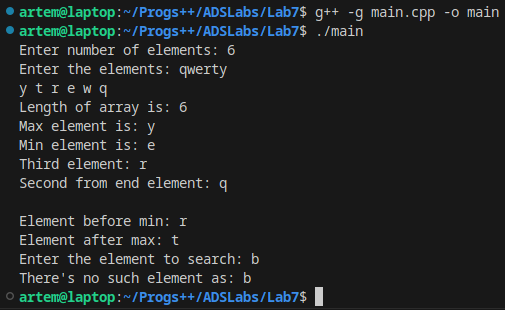
\includegraphics[width=0.90\textwidth]{Screenshot_20231101_083711.png}
    \caption{}
\end{figure}
\subsection*{Висновок} 
Мабуть найменш використовувана структура даних, прохід по списку можливий тільки лінійний, 
елементи вставляються тільки спереду, проте маємо константний час вставки. Зазвичай односторонній список є
реалізацією стеку, звичайно якщо використання динамічної пам'яті доцільне.
\end{document}
